\documentclass[]{tufte-handout}

% ams
\usepackage{amssymb,amsmath}

\usepackage{ifxetex,ifluatex}
\usepackage{fixltx2e} % provides \textsubscript
\ifnum 0\ifxetex 1\fi\ifluatex 1\fi=0 % if pdftex
  \usepackage[T1]{fontenc}
  \usepackage[utf8]{inputenc}
\else % if luatex or xelatex
  \makeatletter
  \@ifpackageloaded{fontspec}{}{\usepackage{fontspec}}
  \makeatother
  \defaultfontfeatures{Ligatures=TeX,Scale=MatchLowercase}
  \makeatletter
  \@ifpackageloaded{soul}{
     \renewcommand\allcapsspacing[1]{{\addfontfeature{LetterSpace=15}#1}}
     \renewcommand\smallcapsspacing[1]{{\addfontfeature{LetterSpace=10}#1}}
   }{}
  \makeatother

\fi

% graphix
\usepackage{graphicx}
\setkeys{Gin}{width=\linewidth,totalheight=\textheight,keepaspectratio}

% booktabs
\usepackage{booktabs}

% url
\usepackage{url}

% hyperref
\usepackage{hyperref}

% units.
\usepackage{units}


\setcounter{secnumdepth}{-1}

% citations
\usepackage{natbib}
\bibliographystyle{plainnat}

% pandoc syntax highlighting
\usepackage{color}
\usepackage{fancyvrb}
\newcommand{\VerbBar}{|}
\newcommand{\VERB}{\Verb[commandchars=\\\{\}]}
\DefineVerbatimEnvironment{Highlighting}{Verbatim}{commandchars=\\\{\}}
% Add ',fontsize=\small' for more characters per line
\newenvironment{Shaded}{}{}
\newcommand{\AlertTok}[1]{\textcolor[rgb]{1.00,0.00,0.00}{\textbf{#1}}}
\newcommand{\AnnotationTok}[1]{\textcolor[rgb]{0.38,0.63,0.69}{\textbf{\textit{#1}}}}
\newcommand{\AttributeTok}[1]{\textcolor[rgb]{0.49,0.56,0.16}{#1}}
\newcommand{\BaseNTok}[1]{\textcolor[rgb]{0.25,0.63,0.44}{#1}}
\newcommand{\BuiltInTok}[1]{#1}
\newcommand{\CharTok}[1]{\textcolor[rgb]{0.25,0.44,0.63}{#1}}
\newcommand{\CommentTok}[1]{\textcolor[rgb]{0.38,0.63,0.69}{\textit{#1}}}
\newcommand{\CommentVarTok}[1]{\textcolor[rgb]{0.38,0.63,0.69}{\textbf{\textit{#1}}}}
\newcommand{\ConstantTok}[1]{\textcolor[rgb]{0.53,0.00,0.00}{#1}}
\newcommand{\ControlFlowTok}[1]{\textcolor[rgb]{0.00,0.44,0.13}{\textbf{#1}}}
\newcommand{\DataTypeTok}[1]{\textcolor[rgb]{0.56,0.13,0.00}{#1}}
\newcommand{\DecValTok}[1]{\textcolor[rgb]{0.25,0.63,0.44}{#1}}
\newcommand{\DocumentationTok}[1]{\textcolor[rgb]{0.73,0.13,0.13}{\textit{#1}}}
\newcommand{\ErrorTok}[1]{\textcolor[rgb]{1.00,0.00,0.00}{\textbf{#1}}}
\newcommand{\ExtensionTok}[1]{#1}
\newcommand{\FloatTok}[1]{\textcolor[rgb]{0.25,0.63,0.44}{#1}}
\newcommand{\FunctionTok}[1]{\textcolor[rgb]{0.02,0.16,0.49}{#1}}
\newcommand{\ImportTok}[1]{#1}
\newcommand{\InformationTok}[1]{\textcolor[rgb]{0.38,0.63,0.69}{\textbf{\textit{#1}}}}
\newcommand{\KeywordTok}[1]{\textcolor[rgb]{0.00,0.44,0.13}{\textbf{#1}}}
\newcommand{\NormalTok}[1]{#1}
\newcommand{\OperatorTok}[1]{\textcolor[rgb]{0.40,0.40,0.40}{#1}}
\newcommand{\OtherTok}[1]{\textcolor[rgb]{0.00,0.44,0.13}{#1}}
\newcommand{\PreprocessorTok}[1]{\textcolor[rgb]{0.74,0.48,0.00}{#1}}
\newcommand{\RegionMarkerTok}[1]{#1}
\newcommand{\SpecialCharTok}[1]{\textcolor[rgb]{0.25,0.44,0.63}{#1}}
\newcommand{\SpecialStringTok}[1]{\textcolor[rgb]{0.73,0.40,0.53}{#1}}
\newcommand{\StringTok}[1]{\textcolor[rgb]{0.25,0.44,0.63}{#1}}
\newcommand{\VariableTok}[1]{\textcolor[rgb]{0.10,0.09,0.49}{#1}}
\newcommand{\VerbatimStringTok}[1]{\textcolor[rgb]{0.25,0.44,0.63}{#1}}
\newcommand{\WarningTok}[1]{\textcolor[rgb]{0.38,0.63,0.69}{\textbf{\textit{#1}}}}

% longtable

% multiplecol
\usepackage{multicol}

% strikeout
\usepackage[normalem]{ulem}

% morefloats
\usepackage{morefloats}


% tightlist macro required by pandoc >= 1.14
\providecommand{\tightlist}{%
  \setlength{\itemsep}{0pt}\setlength{\parskip}{0pt}}

% title / author / date
\title{Visualisation of the German Census Data}
\author{Robin Kohrs}
\date{28-01-2020}


\begin{document}

\maketitle




\begin{center}\rule{0.5\linewidth}{\linethickness}\end{center}

\hypertarget{xaringan}{%
\section{Xaringan}\label{xaringan}}

\begin{itemize}
\tightlist
\item
  Ermöglicht es mit RMarkdown-Syntax Präsentationen zu erstellen
\item
  Basiert auf dem JavaScript-tool \texttt{remark.js}
\item
  RStudio addin ``Infinite Moon Reader'' erstellt Live-Updates bei
  Änderungen im RMarkdown-Dokuement
\end{itemize}

\begin{Shaded}
\begin{Highlighting}[]
\OtherTok{---}
\FunctionTok{title:}\AttributeTok{ }\StringTok{"A  Presentation"}
\FunctionTok{output:}
\NormalTok{  xaringan:}\FunctionTok{:moon_reader:}
    \FunctionTok{yolo:}\AttributeTok{ }\CharTok{true}
\OtherTok{---}
\end{Highlighting}
\end{Shaded}

\begin{marginfigure}

\includegraphics[width=3.56in]{img/logo} \caption[ ]{ }\label{fig:unnamed-chunk-2}
\end{marginfigure}

\begin{marginfigure}
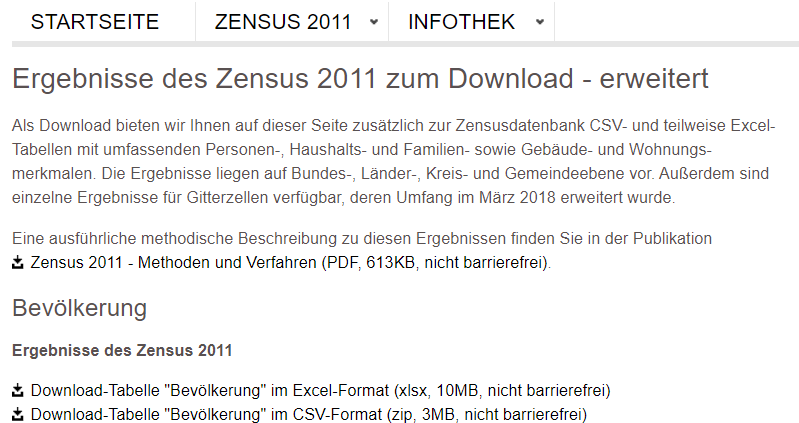
\includegraphics[width=11.1in]{img/ergebnisse} \caption[Quelle]{Quelle: zensus2011.de}\label{fig:unnamed-chunk-3}
\end{marginfigure}

\hypertarget{der-zensus-und-seine-daten}{%
\section{der Zensus und seine Daten}\label{der-zensus-und-seine-daten}}

\begin{itemize}
\tightlist
\item
  letzter durchgeführter Zensus in 2011 (nächster in 2021)
\item
  Daten zu Bevölkerung, Erwerbstätigkeit, Gebäude- und WOhnungsbestand
  häufig in .csv-format
\item
  Gittenzellenbasierte Ergebnisse entweder im 100m-Gitter oder
  1km-Gitter
\end{itemize}

\hypertarget{das-raster-package}{%
\section{\texorpdfstring{das
\texttt{raster}-package}{das raster-package}}\label{das-raster-package}}

\begin{itemize}
\tightlist
\item
  Entwickelt von Robert Hijman in 2010 (das \texttt{sp}-paket wurde 2005
  veröffentlicht)
\item
  \texttt{RasterLayer}, \texttt{RasterBrick} und \texttt{RasterStack}
  sind die zentralen Objekte
\end{itemize}

\begin{Shaded}
\begin{Highlighting}[]
\NormalTok{x =}\StringTok{ }\KeywordTok{raster}\NormalTok{(}\DataTypeTok{ncol=}\DecValTok{36}\NormalTok{, }\DataTypeTok{nrow=}\DecValTok{18}\NormalTok{, }\DataTypeTok{xmn=}\OperatorTok{-}\DecValTok{1000}\NormalTok{, }\DataTypeTok{xmx=}\DecValTok{1000}\NormalTok{, }\DataTypeTok{ymn=}\OperatorTok{-}\DecValTok{100}\NormalTok{, }\DataTypeTok{ymx=}\DecValTok{900}\NormalTok{)}
\KeywordTok{res}\NormalTok{(x) <-}\StringTok{ }\DecValTok{100}
\KeywordTok{projection}\NormalTok{(x) <-}\StringTok{ "+proj=utm +zone=48 +datum=WGS84"} 
\end{Highlighting}
\end{Shaded}

\hypertarget{beispiel}{%
\section{Beispiel}\label{beispiel}}

\renewcommand\refname{References}
\bibliography{lib.bib}



\end{document}
